\documentclass[tikz]{standalone}
\usepackage{pgfplots}
\pgfplotsset{compat=1.15}
\usepackage{mathrsfs}
\usetikzlibrary{arrows,calc}
\usepackage{tkz-euclide}

\pagestyle{empty}

\definecolor{AngleClr}{rgb}{0,0.39215686274509803,0}
\definecolor{ShapeClr}{rgb}{0.6,0.2,0}

\begin{document}

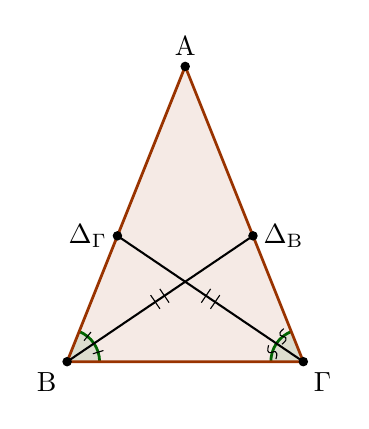
\begin{tikzpicture}[scale=.75]
\tkzSetUpLine[line width=1pt,color=black]
\tkzSetUpPoint[fill=black]

\tkzDefPoints{0/0/B,2/5/A,4/0/C}

\tkzDefLine[bisector](A,B,C) \tkzGetPoint{x}
\tkzDefLine[bisector](A,C,B) \tkzGetPoint{y}

\tkzInterLL(A,C)(B,x) \tkzGetPoint{DB}
\tkzInterLL(A,B)(C,y) \tkzGetPoint{DC}

\tkzFillPolygon[fill=ShapeClr,fill opacity=0.1](A,B,C)

\tkzFillAngles[fill=AngleClr,size=.55,fill opacity=0.1](DB,B,A C,B,DB A,C,DC DC,C,B)
\tkzMarkAngles[mark=|,mksize=2,line width=1pt,size=.55,color=AngleClr](DB,B,A C,B,DB)
\tkzMarkAngles[mark=s,mksize=2,line width=1pt,size=.55,color=AngleClr](A,C,DC DC,C,B)

\tkzDrawSegments[line width=0.75pt,color=black](B,DB C,DC)

\tkzDrawPolygon[color=ShapeClr](A,B,C)

\tkzDrawPoints[size=3](A,B,C,DB,DC)

\tkzLabelPoint[above](A){$\rm A$}
\tkzLabelPoint[below left](B){$\rm B$}
\tkzLabelPoint[below right](C){$\rm \Gamma$}

\tkzLabelPoint[right](DB){$\rm \Delta_B$}
\tkzLabelPoint[left](DC){$\rm \Delta_\Gamma$}

\tkzMarkSegments[mark=||,size=3](B,DB C,DC)

\end{tikzpicture}
\end{document}
